\documentclass{beamer}
    \usetheme{Boadilla}
\usepackage{polyglossia}
    \setmainlanguage{german}
\usepackage{fontspec}
    \setsansfont{Linux Biolinum O}
\usepackage{graphicx}
\usepackage{xcolor}
\usepackage{listings}
    \lstset{language=bash,
	basicstyle=\footnotesize\ttfamily\tiny,
	breaklines=true,
	framextopmargin=50pt,
	frame=bottomline,
	backgroundcolor=\color{white!86!black},
	commentstyle=\color{blue},
	keywordstyle=\color{red},
	stringstyle=\color{orange!80!black}}
\usepackage{amsmath}
\usepackage{amssymb}
\usepackage{siunitx}
\usepackage{booktabs}
\usepackage{float}
\usepackage{tabularx}
\usepackage{caption}
\usepackage{subfig}
\usepackage{tikz}
\usepackage{hyperref}
     \hypersetup{
     colorlinks=true,
     linkcolor=black,
     filecolor=magenta}

\title{\texorpdfstring{\color{blue!50!black}\textbf{Status report - [Date Here] }}{}}
\subtitle{Alignment and Error}
\author{Maurice Donner}
\date{}

\begin{document}

\maketitle

\begin{frame}{Previously...}
Last week: First look at alignment of planes in python, by taking mean hit offset\\
\begin{figure}[H]
    \centering
    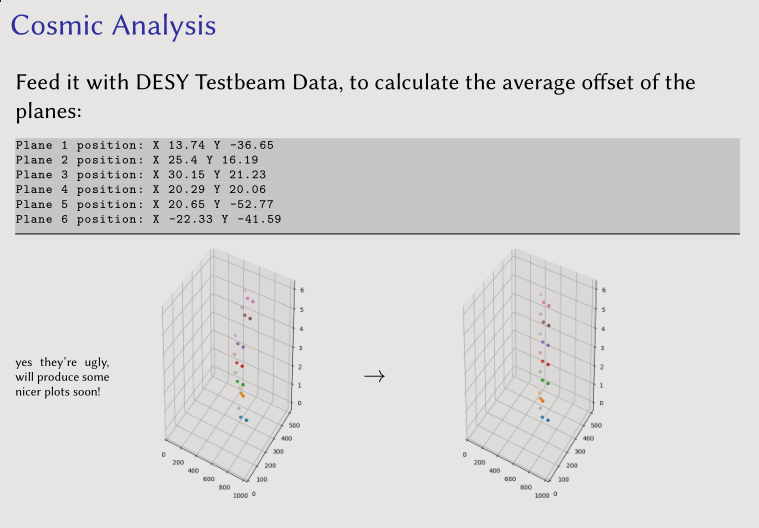
\includegraphics[width=6cm]{Last_Week.png}
    \tiny \ [Status Report - Wednesday, July 9th]
\end{figure}
\pause
This Week: Differences in alignment from 2019 and 2020 Testbeam data
\end{frame}

\begin{frame}[fragile]{Alignment Error}
    \LARGE Idea: \normalsize \\
    Look at standard deviation of hit offset, to see if comparison between two
    testbeam runs are inside of the margin of error \\[.3cm]
    \LARGE First Look: \normalsize Huge \( \sigma \) \\
    \begin{lstlisting}
Plane 1 position: X 26.35 +- 21.04 Y -48.79 +- 16.43
Plane 2 position: X 25.9 +- 21.02 Y 17.13 +- 14.94
Plane 3 position: X 30.61 +- 21.8 Y 21.26 +- 16.02
Plane 4 position: X 20.94 +- 22.31 Y 20.2 +- 16.7
Plane 5 position: X 19.42 +- 25.1 Y -54.09 +- 19.62
Plane 6 position: X -24.11 +- 24.77 Y -43.44 +- 19.12
    \end{lstlisting}
\end{frame}
\begin{frame}[fragile]{Alignment Error}
    \LARGE First Look: \normalsize Huge \( \sigma \) 
    \begin{lstlisting}
Plane 1 position: X 26.35 +- 21.04 Y -48.79 +- 16.43
Plane 2 position: X 25.9 +- 21.02 Y 17.13 +- 14.94
Plane 3 position: X 30.61 +- 21.8 Y 21.26 +- 16.02
Plane 4 position: X 20.94 +- 22.31 Y 20.2 +- 16.7
Plane 5 position: X 19.42 +- 25.1 Y -54.09 +- 19.62
Plane 6 position: X -24.11 +- 24.77 Y -43.44 +- 19.12
    \end{lstlisting}
    \begin{minipage}{.49\textwidth}
	\begin{figure}[H]
	\centering
	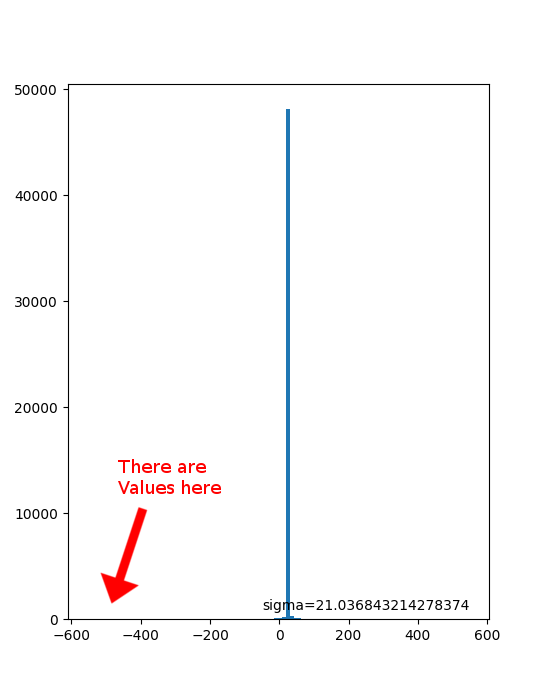
\includegraphics[trim=0 0 0 50, clip, width=.8\textwidth]{Beforeimasked_Witharrow.png}
	\end{figure}
    \end{minipage}
    \begin{minipage}{.49\textwidth}
	\begin{figure}[H]
	\centering
	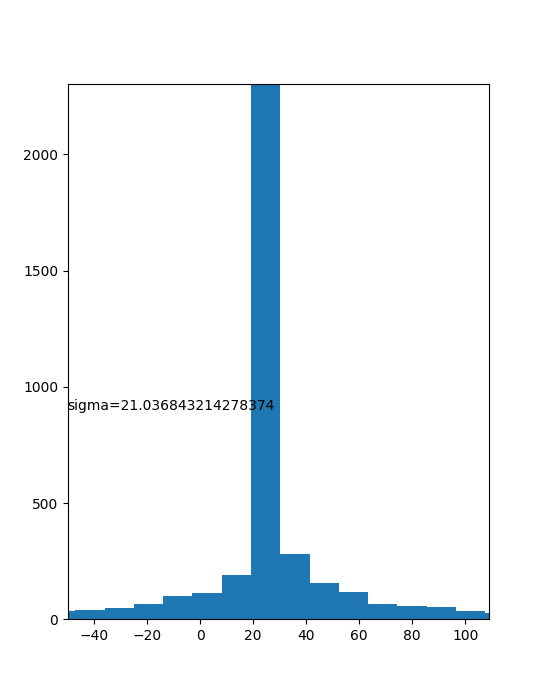
\includegraphics[trim=0 0 0 50, clip, width=.8\textwidth]{Beforeimasked_zoom.png}
	\end{figure}
    \end{minipage}
\end{frame}

\begin{frame}{Alignment Error}
    \LARGE Suspicion: \normalsize Particles, that have suffered from large-
    angle scattering will produce high deviation in hit position.\\ \pause
    \( \rightarrow \) define an area, to where if the particle has scattered
    outside of this area, the track belonging to that event will not be used
    for alignment.\\
    \( \rightarrow \) For now, defined a square of \( 20 \times 20 \) pixels
    around the expected mean. \pause
    \begin{figure}[H]
	\centering
	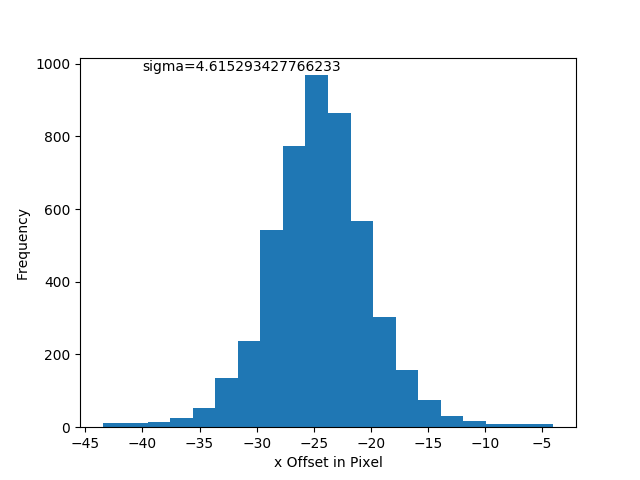
\includegraphics[trim=0 0 0 40,clip,width=6.3cm]{Afterimasked.png}
    \end{figure}
\end{frame}

\begin{frame}[fragile]{Comparing the DESY-Runs from 2019 and 2020}
    \begin{minipage}{.49\textwidth}
	\begin{lstlisting}
                     2019
Aligning planes...
Masked 2565 hits
Plane 1 : X 26.49 +- 1.56 Y -49.55 +- 1.57
Masked 2794 hits
Plane 2 : X 26.00 +- 2.28 Y 17.34 +- 2.42
Masked 3036 hits
Plane 3 : X 30.74 +- 2.80 Y 21.66 +- 2.7
Masked 3090 hits
Plane 4 : X 20.93 +- 3.41 Y 20.59 +- 3.22
Masked 3431 hits
Plane 5 : X 19.26 +- 3.98 Y -55.17 +- 3.71
Masked 3652 hits
Plane 6 : X -24.43 +- 4.61 Y -44.41 +- 4.25
\end{lstlisting}
    \end{minipage}
    \begin{minipage}{.49\textwidth}
	\begin{lstlisting}
                     2020
Aligning planes...
Masked 5390 hits
Plane 1 : X 10.89 +- 2.34 Y -46.93 +- 2.45
Masked 5628 hits
Plane 2 : X 6.06 +- 2.70 Y 11.77 +- 2.88
Masked 6142 hits
Plane 3 : X -0.41 +- 3.09 Y 6.92 +- 3.21
Masked 6694 hits
Plane 4 : X -25.89 +- 3.57 Y 8.00 +- 3.50
Masked 7347 hits
Plane 5 : X -28.06 +- 4.09 Y -34.12 +- 4.05
Masked 7681 hits
Plane 6 : X -79.91 +- 4.61 Y -19.14 +- 4.48
\end{lstlisting}
    \end{minipage}
    \pause
    \begin{figure}[H]
	\centering
	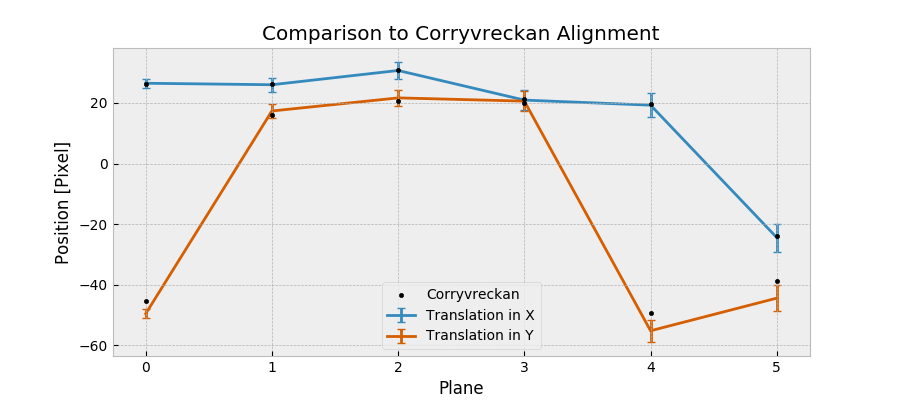
\includegraphics[trim=0 0 0 18,clip,width=9cm]{Corry.png}
    \end{figure}
\end{frame}
\begin{frame}[fragile]{Comparing the DESY-Runs from 2019 and 2020}
    \begin{minipage}{.49\textwidth}
	\begin{lstlisting}
                     2019
Aligning planes...
Masked 2565 hits
Plane 1 : X 26.49 +- 1.56 Y -49.55 +- 1.57
Masked 2794 hits
Plane 2 : X 26.00 +- 2.28 Y 17.34 +- 2.42
Masked 3036 hits
Plane 3 : X 30.74 +- 2.80 Y 21.66 +- 2.7
Masked 3090 hits
Plane 4 : X 20.93 +- 3.41 Y 20.59 +- 3.22
Masked 3431 hits
Plane 5 : X 19.26 +- 3.98 Y -55.17 +- 3.71
Masked 3652 hits
Plane 6 : X -24.43 +- 4.61 Y -44.41 +- 4.25
\end{lstlisting}
    \end{minipage}
    \begin{minipage}{.49\textwidth}
	\begin{lstlisting}
                     2020
Aligning planes...
Masked 5390 hits
Plane 1 : X 10.89 +- 2.34 Y -46.93 +- 2.45
Masked 5628 hits
Plane 2 : X 6.06 +- 2.70 Y 11.77 +- 2.88
Masked 6142 hits
Plane 3 : X -0.41 +- 3.09 Y 6.92 +- 3.21
Masked 6694 hits
Plane 4 : X -25.89 +- 3.57 Y 8.00 +- 3.50
Masked 7347 hits
Plane 5 : X -28.06 +- 4.09 Y -34.12 +- 4.05
Masked 7681 hits
Plane 6 : X -79.91 +- 4.61 Y -19.14 +- 4.48
\end{lstlisting}
    \end{minipage}
    \begin{figure}[H]
	\centering
	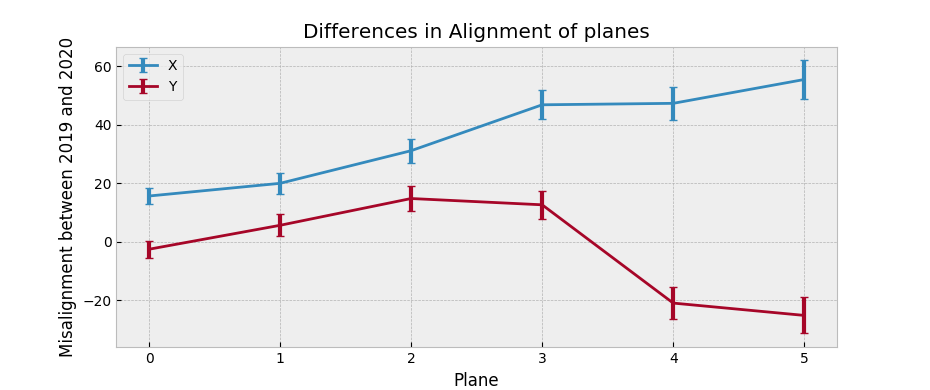
\includegraphics[trim=0 0 0 18,clip,width=9cm]{Misalignment.png}
    \end{figure}
\end{frame}

\end{document}
